\documentclass{article}

\usepackage[utf8]{inputenc}
\usepackage{setspace}
\usepackage{geometry}
\usepackage{graphicx}
\usepackage{caption}
\usepackage{indentfirst}
\usepackage{anyfontsize}
\usepackage{textcomp}
\usepackage{lipsum}
\usepackage{float}
\usepackage{changepage}
\usepackage [english]{babel}
\usepackage [autostyle, english = american]{csquotes}
\MakeOuterQuote{"}

\graphicspath{}



\title{ODE Modeling}
\author{Geneva Porter}
\date{9 October 2018}

%\begin{figure}[H]
%\centering{\includegraphics[width=10cm]{FILENAME.eps}}
%	\caption{CAPTION}
%\end{figure}

%$\begin{bmatrix}
%11      & 12  \\
%21      & 22  \\
%\end{bmatrix}$

\begin{document}
	
\begin{titlepage}
\maketitle
\thispagestyle{empty}


\begin{center}
	
\large \it San Diego State University 
	
Professor J Mahaffy, Math 636

\end{center}
\end{titlepage}

\section*{Problem 4, Cat Detective}

d. Figure 1 shows the three model for environmental temperature. A constant temperature, in this case $t=$14.5$\cdot$C, is much simpler to implement in a model, but not realistic. Obviously factors like sunlight and weather patterns will change the temperature continually. The linear model for temperature, $T(t)=14.5-0.6t$, is only slightly more realistic. Outside the domain we are examining, however, such a model is even less logical than a constant temperature. Keeping the linear model would show no increase in temperature, eventually passing absolute zero. Using this model to predict temperature would imply that it was $20\cdot C$ around 10pm, which may be too warm for a climate that reached 14.5$\cdot$C by 7am. We can see that the y-intercept of the linear model is significantly higher that the other two. The trigonomic model is far superior to the other two. It implies that the temperature increases through the morning and decreases in the evening cyclically. This most closely resembles actual temperature variations over a long period of time.

\begin{figure}[H]
	\centering{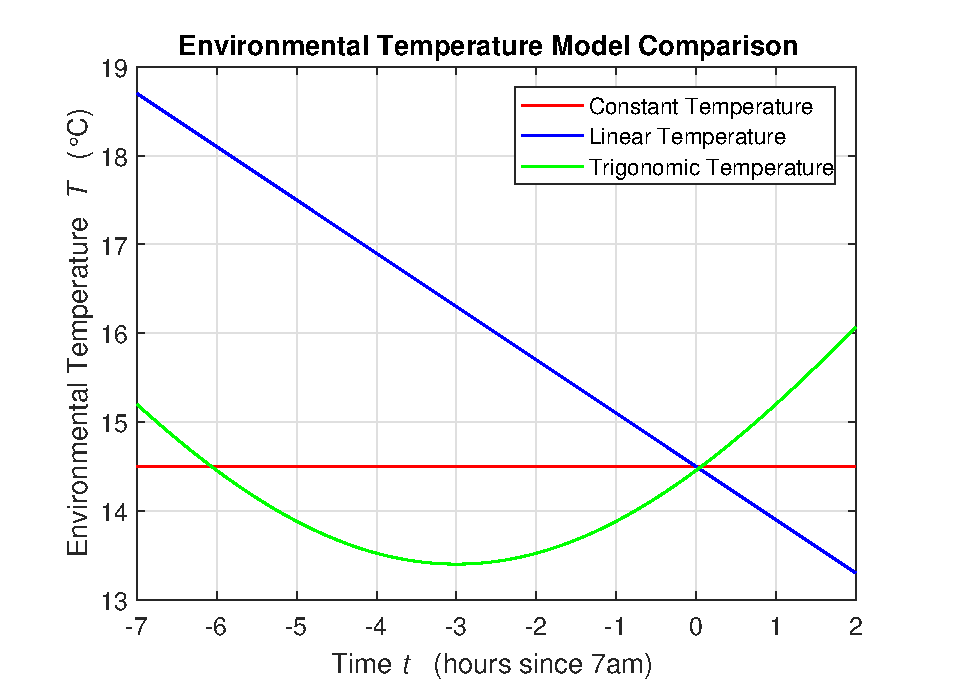
\includegraphics[width=15cm]{f1.eps}}
	\caption*{Figure 1}
\end{figure}

e. Figure 2 is a comparison of the predicted time of death using each environmental temperature model. Each prediction is within a 45-minute interval. Without knowing the actual time of death, it is difficult to say which model yields the most accurate result. Based on the discussion in part (d.), the trigonomic model is likely the most accurate. It predicts a time of death later than the other two, which may imply that the linear temperature model is the least accurate. Even though the temperature models differ significantly, the predicted times of death do not. One improvement to the linear model might be do decrease the slope so that it would better coencide with the actual temperature from the night before. 

\begin{figure}[H]
	\centering{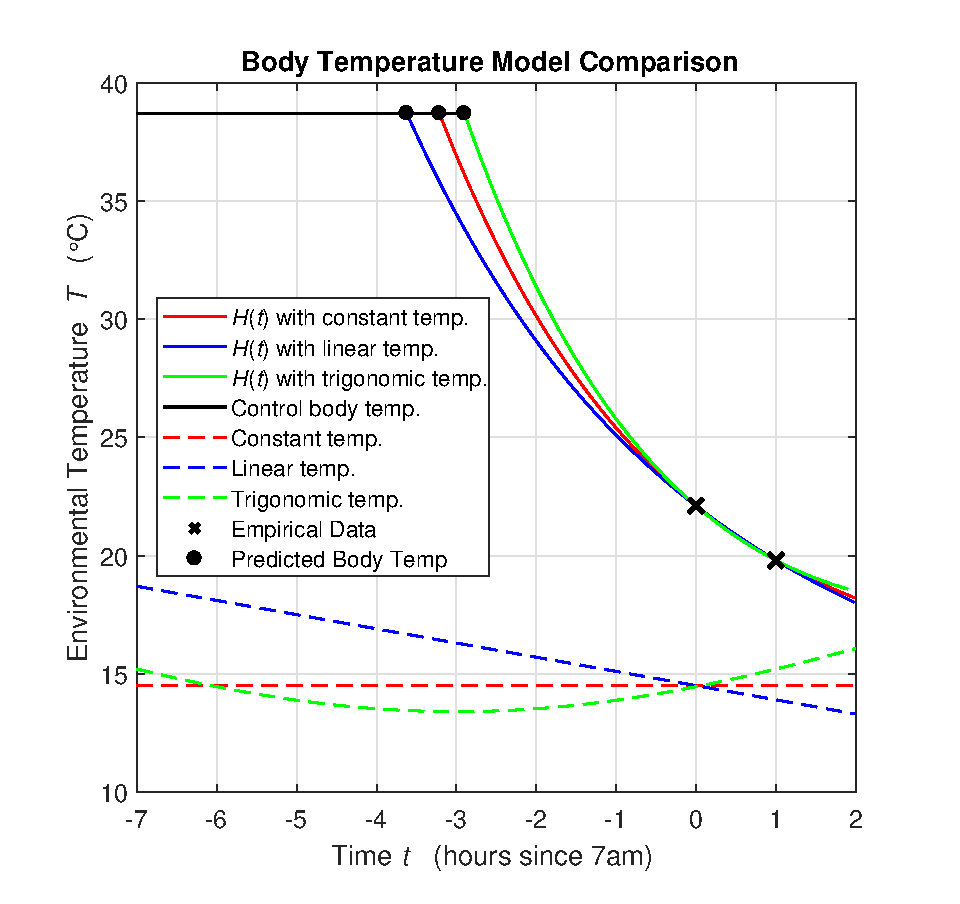
\includegraphics[width=15cm]{f2.eps}}
	\caption*{Figure 2}
\end{figure}

\pagebreak

\section*{Problem 5, Blue Marlin Size}

b. As shown below in Figure 3, the rate of growth for the Blue Marlin decreases with time. The rate approaches zero as the length function approaches a horizontal asymptote of about 3.8 meters. This implies that the maximum length for the Blue Marlin is about 3.8 meters. The model simulates that data very well, shown by a small sum of squared errors (SSE$\approx$0.01).

d. Figure 4 (below) shows how the length of a Blue Marlin correlates to its weight. We can see that the rate of weight gain is increasing, and realistically the weight itself reaches a maximum only by being bounded by its maximum length. A Blue Marlin that would be able to reach a maximum length of 3.8 meters would then weigh nearly 900 kg, the size of a small whale. The data fits this model reasonably well, with a sum of squared errors at about 823.

\begin{figure}[H]
	\centering{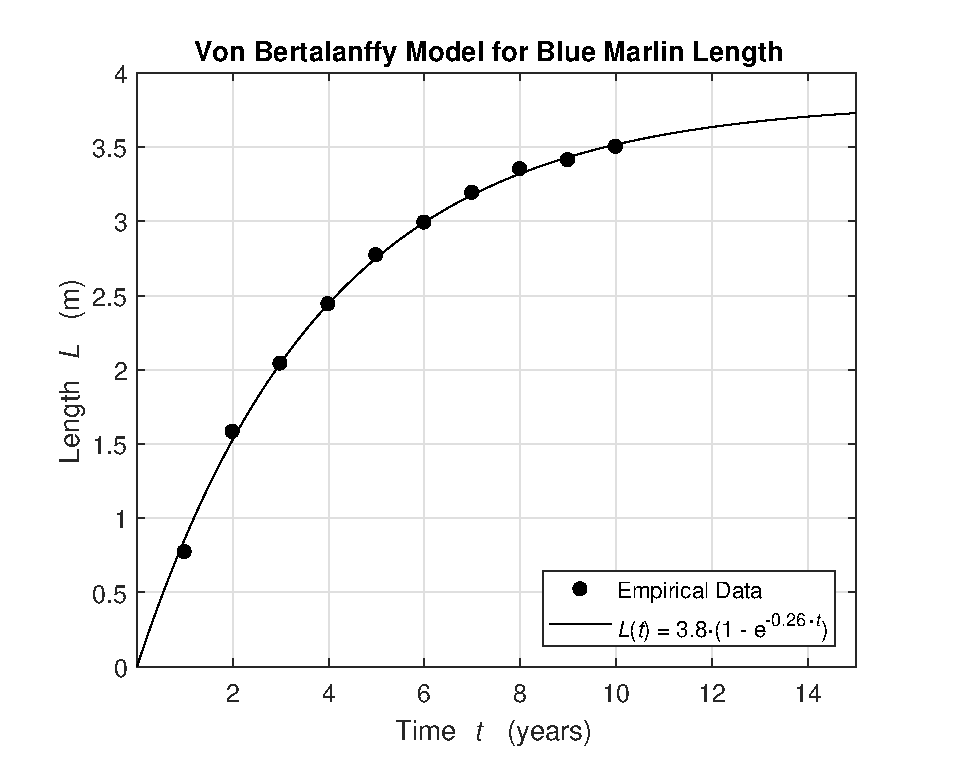
\includegraphics[width=15cm]{f3.eps}}
	\caption*{Figure 3}
\end{figure}

\begin{figure}[H]
	\centering{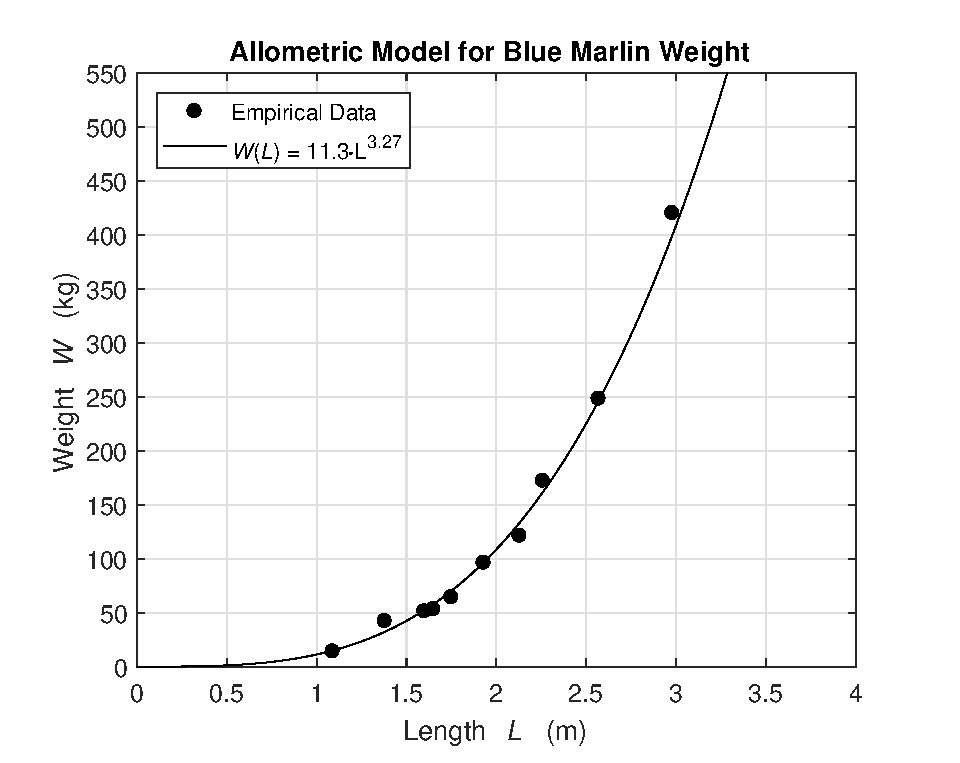
\includegraphics[width=15cm]{f4.eps}}
	\caption*{Figure 4}
\end{figure}



f. Below is a composite model for predicting the weight of a Blue Marlin over time. We can see that this graph also has a horizontal asymptote for the maximum weight corresponding the the value of the maximum length. The derivative is in red and shows the rate of weight gain, with the maximum representing the inflection point of the function at about 4.9 years. At that time, the rate of weight gain begins to decrease and approaches zero at the horizontal asymptote. My modeling efforts seem to have yielded fairly accurate representations in this lab, so I am inclined to trust that the composite model would be accurate as well. It also seems to work well over long term projections, as the horizontal asymptote enforces a weight capacity. One weakness that may be present in the weight vs. time model is that an abnormally long Blue Marlin would probably not weigh much more than the modeled maximum weight--it would seem probable that a 4 meter fish could be found, but highly improbable that it would weigh over 1000kg. This weakness is eliminated in the composite function, as the weight is now bounded by the maximum length.

\begin{figure}[H]
	\centering{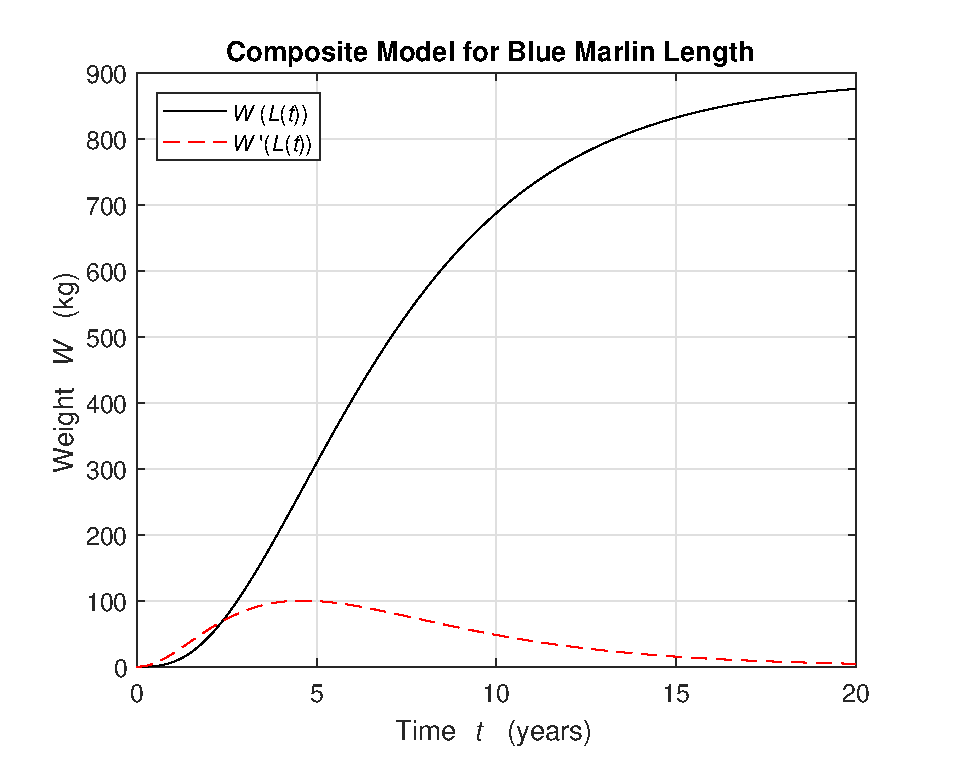
\includegraphics[width=15cm]{f5.eps}}
	\caption*{Figure 5}
\end{figure}

\section*{Problem 6, Allee Effect}

b. This is a phase portrait of a model incorporating the allee effect. We can see that there are 3 equilibria; an extinction at 0, a threshold at about 5, and a carrying capacity around 9. The threshold separates the tendency of the population to go towards extinction or towards carrying capacity. The logistic model, on the other hand, only has 2 equilibria: at 0 and at the carrying capacity. Its phase portrait would display a population that would tend toward the carrying capacity and away from zero. One major drawback of the logistic model is that even if the population were 1, it would predict a tendency towards the carrying capacity. This, of course, would only be possible for asexual populations. Accounting for the allee effect is more realistic, as it takes such instances into account. Several species (such as the giant panda mentioned in the homework problem), will not mate if there is not a sufficient number of possible mates. This would be a situation where the population would be below the growth threshold, and would lead to extinction.

\begin{figure}[H]
	\centering{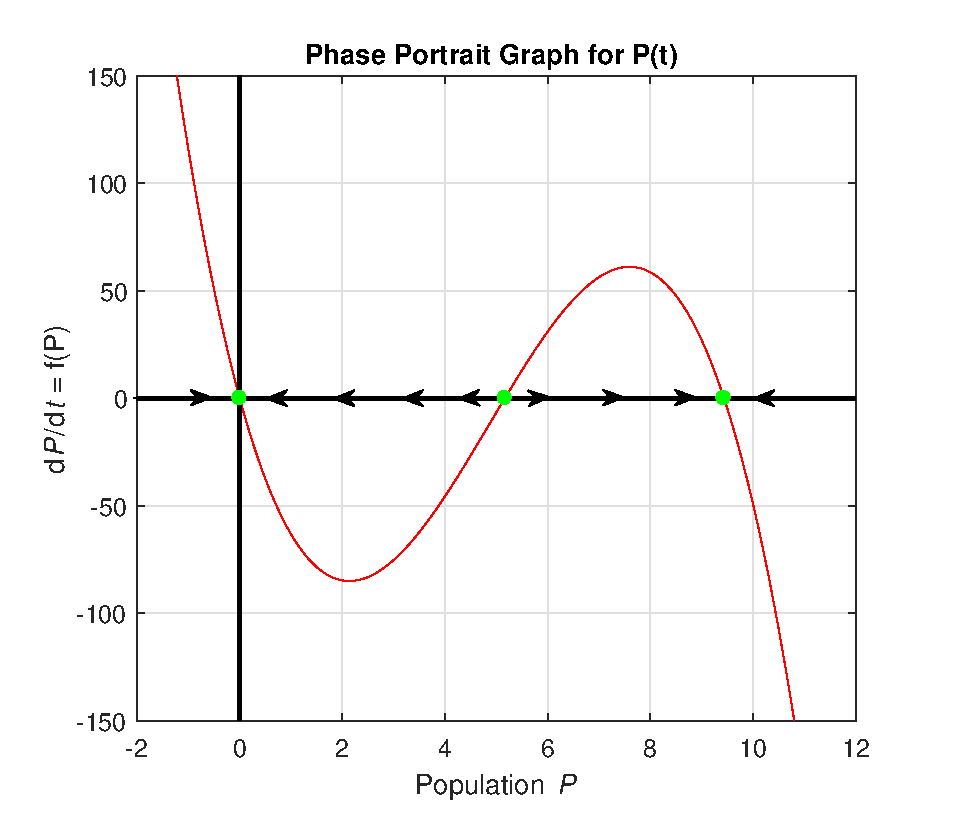
\includegraphics[width=15cm]{f6.eps}}
	\caption*{Figure 6}
\end{figure}

\section*{Problem 7, Competing Species}

a. The two equations given for competing species are:

\begin{center}
	{$dX/dt = 2.4X-5.6X^2+5XY$ and $dY/dy=4.1Y-3.2Y^2+2.9XY$}
\end{center}

For both species, the first coefficient is the Malthusian growth rate, unbounded by carrying capacity. The second coefficient is negative, and helps to account for such issues. It eliminates the part of the population that dies from lack of resources. The third term represents the dynamics between the two species. Since this term is positive, it implies that the existence of species Y will help species X survive and visa versa, so they must not have a hunter-prey relationship. One example of this would be dogs and humans: dogs will guard families and protect the young, while humans will provide them with food and shelter.

e. Ultimately, both species will reach an equilibrium where there are just enough resources to maintain them both. This is assuming that both species are present in sufficient mating numbers at the beginning of the simulation. Also, no species can exist without the other, as the extinction of one causes the other to also tend toward extinction. 

\begin{figure}[H]
	\centering{\includegraphics[width=15cm]{pp2.eps}}
	\caption*{Figure 7}
\end{figure}

\vspace{5mm}

\section*{Worksheet, Competing Beetles}

a. The following 2 graphs show the independent growth of two species of beetles, Rhizopertha ($R$) and Oryzaephilus ($O$). Population data for the first few months was used to model Malthusian growth. Here, the carrying capacity is not considered. We are only modeling the exponential growth that occurs with abundant resources. Here are the solutions to the Malthusian growth model for the first 119 days for $R$ and the first 77 days for $O$:

\begin{center}
$R(t)=18.11e^{0.02304\cdot t}$, SSE=7719

$O(t)=4.369e^{0.05444\cdot t}$, SSE=470.3
\end{center}

\begin{figure}[H]
	\centering{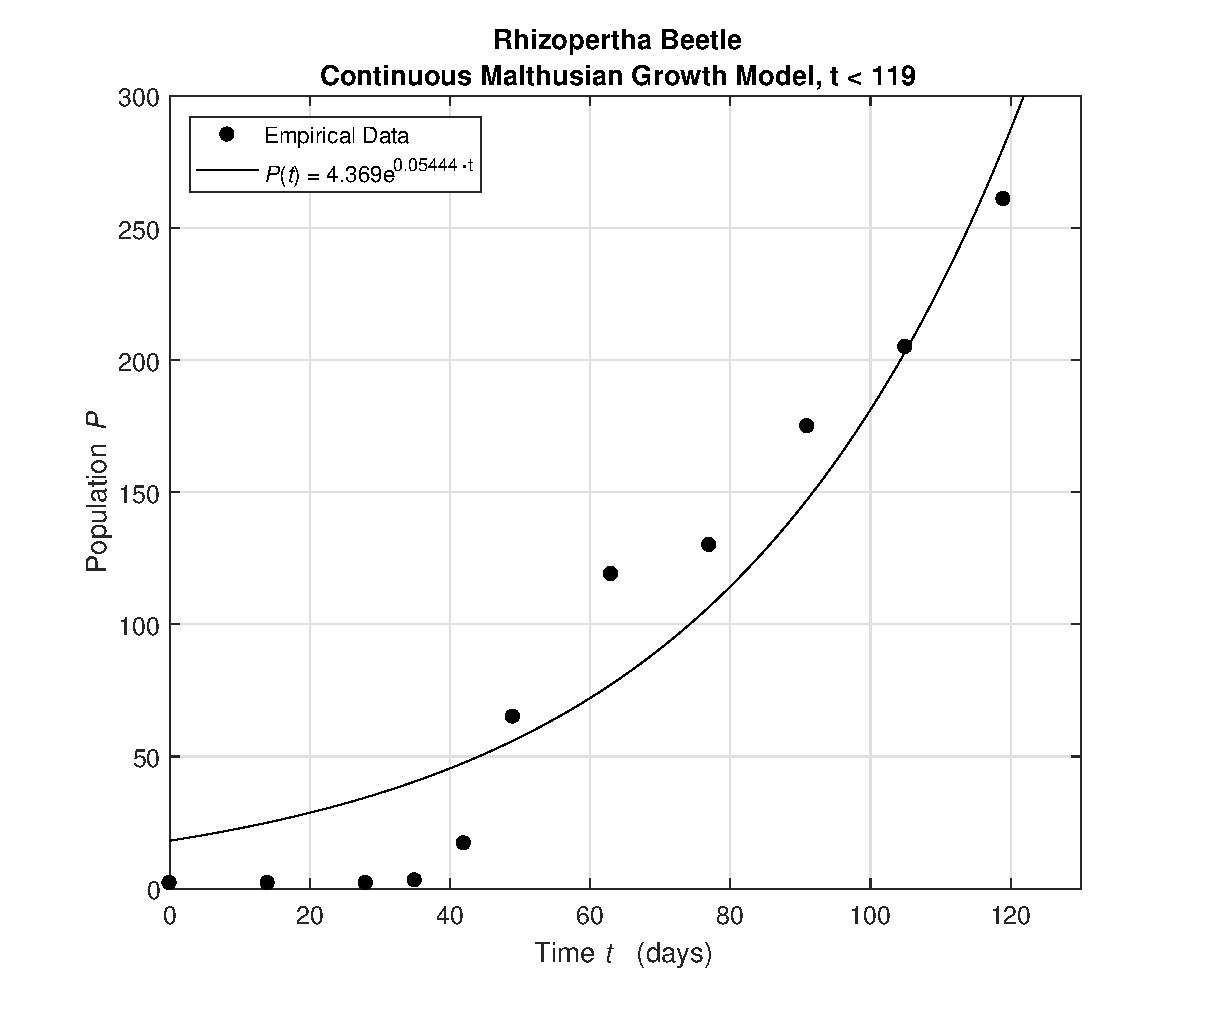
\includegraphics[width=15cm]{f9.eps}}
	\caption*{Figure 8}
\end{figure}

\begin{figure}[H]
	\centering{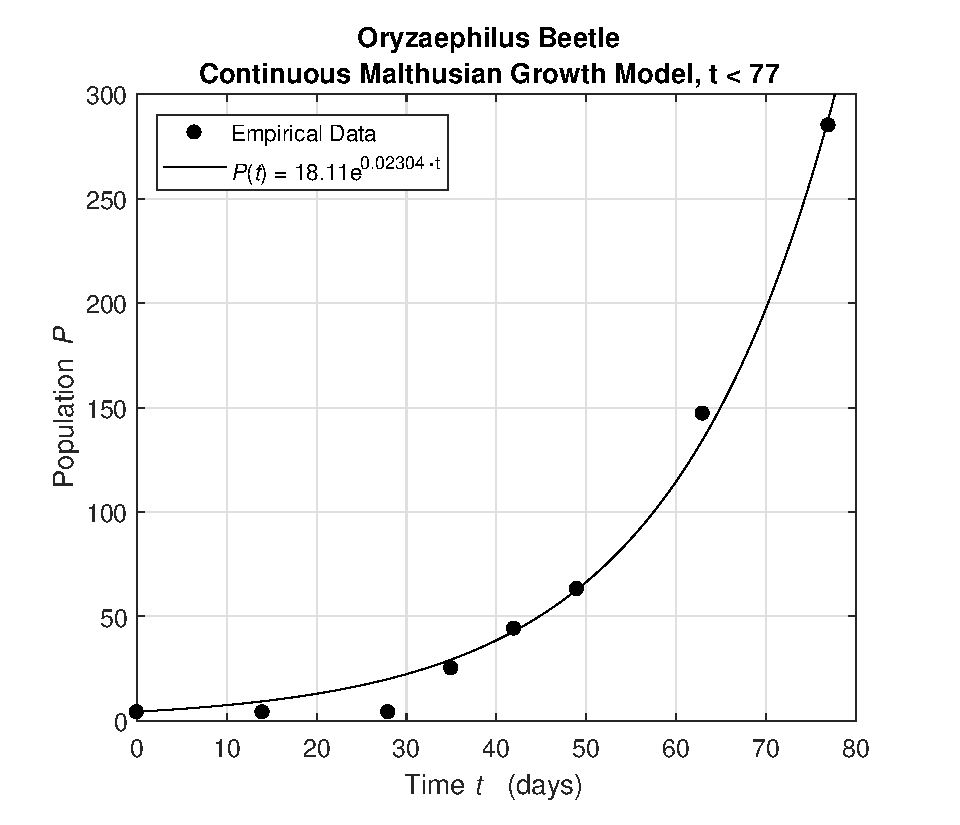
\includegraphics[width=15cm]{f10.eps}}
	\caption*{Figure 9}
\end{figure}

b. Next, we accounted for all the data given for each species and used the logistic model. We used the values for growth rate and initial population found in part (a.) as guesses for parameters $M$, $P_0$, and $r$. Figures 10 and 11 show the graphs of these models. The following are the values found for the logistic growth model:

\begin{center}
	$M_R=337.5869$, $P_R=6.3661$, $r_R=0.0444$, SSE = 4505,
	
	$M_O=442.7694$, $P_O=2.9275$, $r_O=0.0690$, SSE = 8030, 
\end{center}



\begin{figure}[H]
	\centering{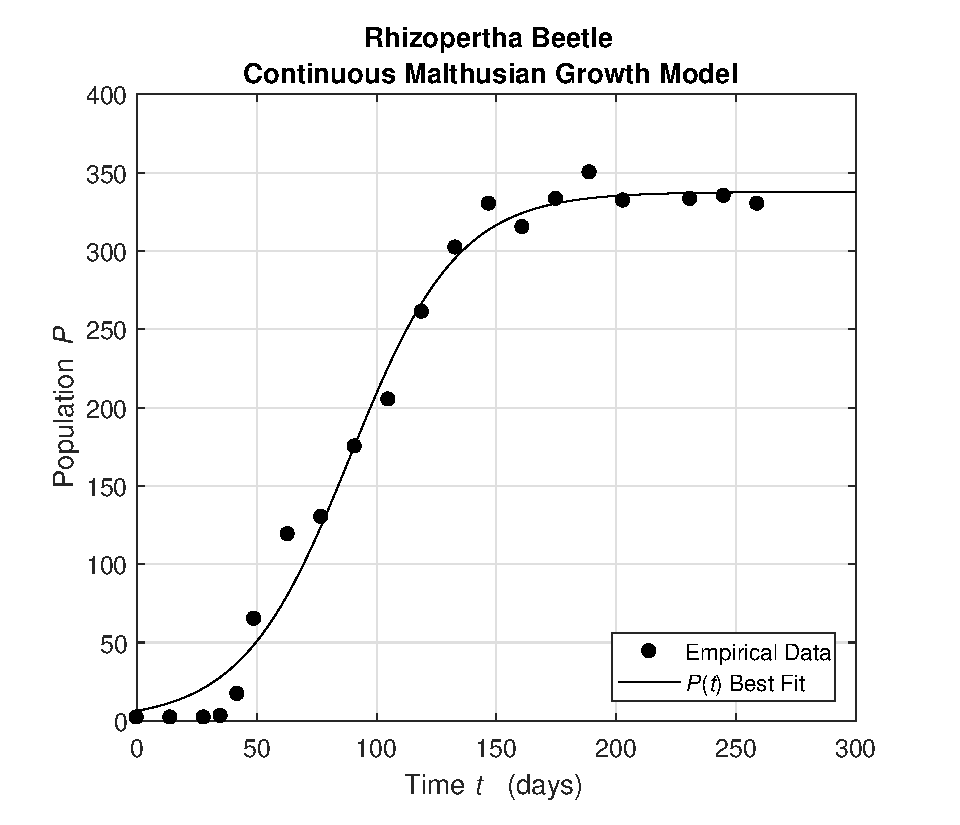
\includegraphics[width=15cm]{f11.eps}}
	\caption*{Figure 10}
\end{figure}

\begin{figure}[H]
	\centering{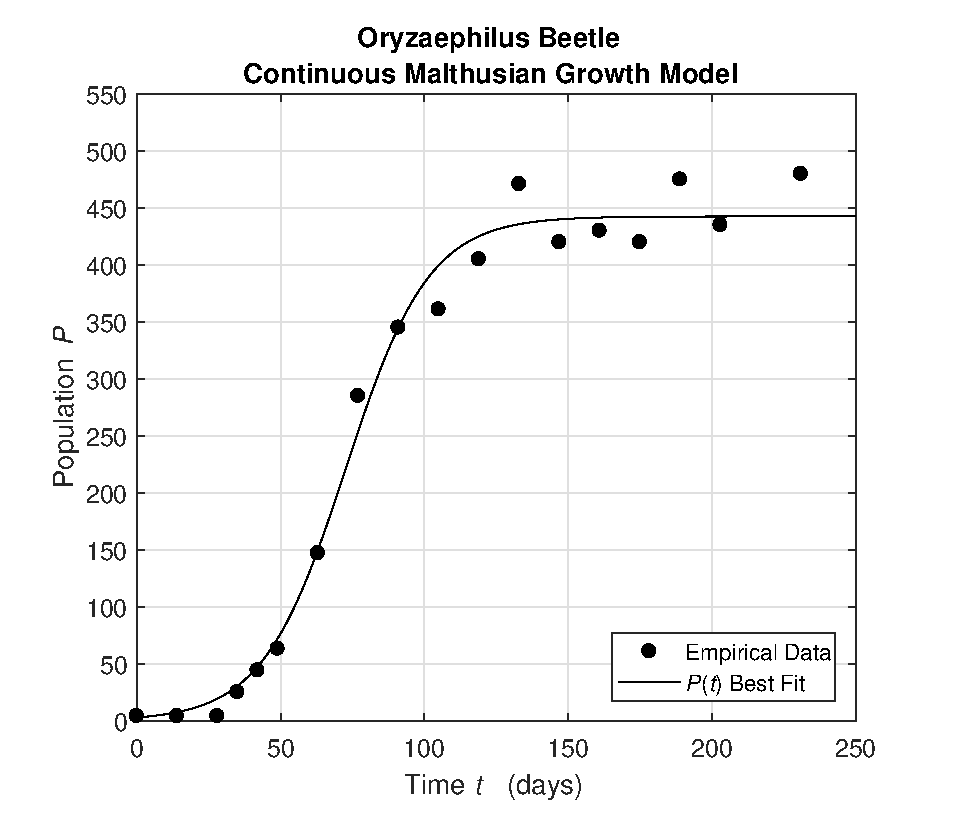
\includegraphics[width=15cm]{f12.eps}}
	\caption*{Figure 11}
\end{figure}

c. For the competing species model, a different data set was used that included population growth measurements with both species present. The differential competing species terms are shown below, and modeled in figure 12.

\begin{center}
	
	$R: a_1=0.02304, a_2=0.0001316, a_3=-0.00002923, SSE\approx21087$
	
	$O: b_1=0.05444, b_2=0.0001559, b_3=-0.00004579, SSE\approx16187$
	
\end{center}


\begin{figure}[H]
	\centering{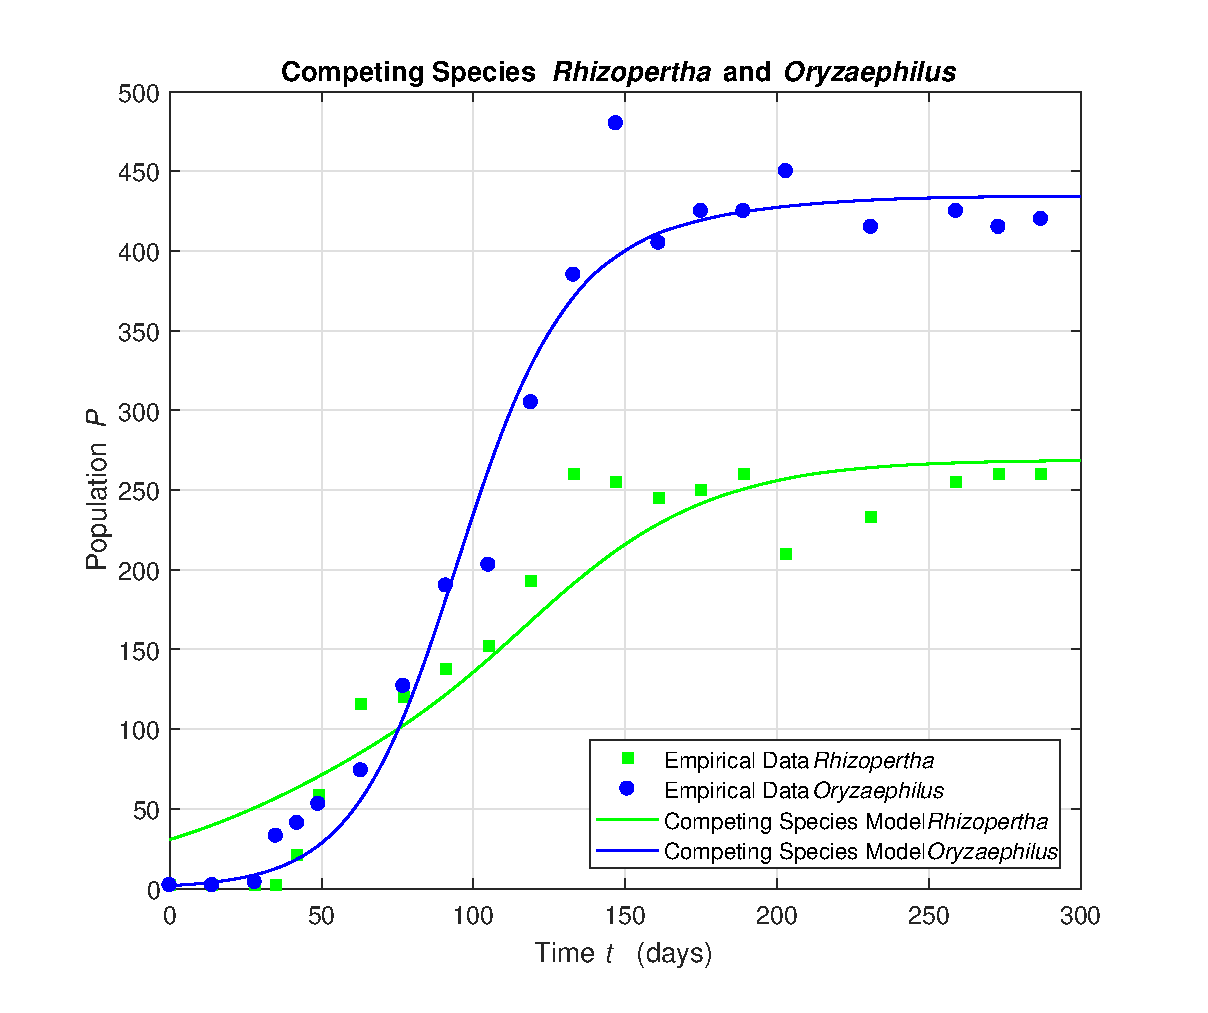
\includegraphics[width=15cm]{f13.eps}}
	\caption*{Figure 12}
\end{figure}
d. For this species, there is a cohabitation equilibria when the populations of $R$ and $O$ are about 270 and 432, respectively. Since these species do not depend on each other, they can reach an equilibrium and stay there if the other species is not present. Notice that in Figure 13, the y-axis has a saddle point around 350. Without the presence of $R$, this node would be stable. Likewise, when there is no $O$ present, $R$ can maintain a population of about 175 as shown by the directional vectors near the x-axis. It is interesting to note that while the ending term for each equation is negative, the species do benefit each other in some way, as the population is greater when both are present. If both species are present, over a long period of time they should remain around 270 for $R$ and 432 for $O$. The equilibria are shown below.


\vspace{5mm}

$\lambda_{(0,0)}=[0.02304,0.05444]$, unstable node.

$\lambda_{(175.03517,0)}=[-0.02304,0.06279]$, saddle node.

$\lambda_{(0,349.2183)}=[-0.05444,0.03315]$, saddle node.

$\lambda_{(269.9702,431.8545)}=[-0.07177,-0.03109]$, stable node.


\begin{figure}[H]
	\centering{\includegraphics[width=15cm]{pp3.eps}}
	\caption*{Figure 13}
\end{figure}

\end{document}





































